\documentclass[12pt]{article}
\usepackage[pdftex]{graphicx}
\usepackage{epstopdf}
\usepackage{amsmath, algorithmic, color, multicol}


\title{Answers to Problem Set 2}
\author{
	Lauren Hinkle (lhinkle)\\
	Pedro d'Aquino  (pdaquino)\\
	Robert Goeddel (rgoeddel)}

\begin{document}
\maketitle
\pagebreak

\section{Graphical Models and Conditional Distributions}

\paragraph{A}
\begin{enumerate}
	\item $u_i$ and $u_{i+1}$ are unconditionally independent, but are dependent given the robot trajectory.
	\item $z_i$ and $z_{i+1}$ are dependent, even given all the positions, because the dependence flows through $L_0$.
	\item If the trajectory of the robot is known, the our posterior estimate of the locations of the
    landmarks is only dependent on the landmark observation noise. For example, if the noise is Gaussian,
    we'd expect the mean of our observations of a particular landmark to converge on the actual location
    of the landmark as we gain more observations. Since our SLAM estimates of these positions would've
    been affected by odometry noise without a known trajectory, we expect our estimates to improve.
\end{enumerate}

\paragraph{B}
\begin{enumerate}
	% Part B1
	\item  Given a binary variable $x\in\{a,b\}$, after one observation $z_1: p(x = a | z_1)$, the probability that $x=a$ in terms of only $p(a)$, $p(z_1| a)$ and $p(z_1 | b)$ is
	\begin{align*}
	p(a|z_1) &= \frac{p(z_1|a)p(a)}{p(z_1)} \\
						&= \frac{p(z_1|a)p(a)}{p(z_1|a)p(a) + p(z_1|b)p(b)} \\
						&= \frac{p(z_1|a)p(a)}{p(z_1|a)p(a) + p(z_1|b)(1-p(a))}
	\end{align*}
	% Part B2 XXX - not sure about p(z_1|z_2), also doesn't align with results in B3
	\item  First we show $p(z_1,z_2|a) = p(z_2|a,z_1)p(z_1|a)p(a)$:
	\begin{align*}
	p(z_1,z_2|a) &= \frac{p(z_1,z_2,a)}{p(a)} \\
			     &= \frac{p(z_2|a,z_1)p(a,z_1)}{p(a)} \\
			     &= \frac{p(z_2|a,z_1)p(z_1|a)p(a)}{p(a)}\\
			     &=p(z_2|a,z_1)p(z_1|a)p(a)
	\end{align*}
	Then the correct expression for the probability of $x$ after two Bayes updates is derived as follows:
	\begin{align*}
	p(a|z_1,z_2) &= \frac{p(z_1,z_2|a)p(a)}{p(z_1,z_2)} \\
			     &= \frac{p(z_2|a,z_1)p(z_1|a)}{p(z_1,z_2)} \\
			     &= \frac{p(z_2|a,z_1)p(z_1|a)p(a)}{p(z_1)p(z_2)}\\
			     &= \frac{p(z_2|a,z_1)p(z_1|a)p(a)}{(p(z_1|a)p(a)+p(z_1|b)p(b))\cdot(p(z_2|a)p(a)+p(z_2|b)p(b))}
	\end{align*}
	This last step can be done because $z_1$ and $z_2$ are independent.  David's mistake occurs when he assumes the independent observations $z_1$ and $z_2$ have equal probability:
	\begin{align*}
	p(a|z_1,z_2) &= \frac{p(z_2|a,z_1)p(z_1|a)p(a)}{p(z_1)p(z_2)} \\
			     &= \frac{p(z_2|a,z_1)p(z_1|a)p(a)}{p(z_1)^2} \\
			     &= \frac{p(z_2|a,z_1)p(z_1|a)p(a)}{(p(z_1|a)p(a)+p(z_1|b)p(b))^2}
	\end{align*}
	% Part B3
	\item  Let $p(z | a) = p(z | b)$.
	\begin{align*}
	p(a,z_1,z_2,z_3,z_4) &= p(a,z_1,z_2,z_3|z_4)p(z_4) \\
					  &=  p(a,z_1,z_2|z_3,z_4)p(z_3|z_4)p(z_4) \\
					  &=  p(a,z_1|z_2,z_3,z_4)p(z_2|z_3,z_4)p(z_3|z_4)p(z_4) \\
					  &=  p(a|z_1,z_2,z_3,z_4)p(z_1|z_2,z_3,z_4)p(z_2|z_3,z_4)p(z_3|z_4)p(z_4) \\
	p(a|z_1,z_2,z_3,z_4) &=	\frac{p(a,z_1,z_2,z_3,z_4)}{p(z_1|z_2,z_3,z_4)p(z_2|z_3,z_4)p(z_3|z_4)p(z_4)} \\
	 				  &=  \frac{p(z_4|a,z_1,z_2,z_3)p(z_3|a,z_1,z_2)p(z_2|a,z_1)p(z_1|a)p(a)}{p(z_1|z_2,z_3,z_4)p(z_2|z_3,z_4)p(z_3|z_4)p(z_4)}
	\end{align*}

    \begin{align*}
    p(z) &= p(z|a)p(a) + p(z|b)p(b) \\
        &= p(z|a)(p(a) + p(b)) \\
        &= p(z|a) \\
    p(a|z) &= \frac{p(z|a)p(a)}{p(z)} \\
        &= \frac{p(z|a)p(a)}{p(z|a)} \\
        &= p(a) \\
    \end{align*}

    From this we claim that $a$ is independent of observations $z$. Thus, given
    any number of observations $z$, we learn no more about $a$, so:

    $p(a|z_1,z_2,z_3,z_4) = p(a)$
\end{enumerate}

%\pagebreak

\section{Matrix Sparsity}

% XXX Assumed reflexive edges? YES / NO?
\paragraph{(i)}
The adjaceny matrix for the given graph looks like:

\begin{tabular}{| c || c | c | c | c | c | c | c | c |}
\hline
& a & b & c & d & e & f & g & h \\
\hline \hline
a & & X & X & & & & & X \\
\hline
b & X & & X & & & & & \\
\hline
c & X & X & & X & X & & & \\
\hline
d & & & X & & X & & & \\
\hline
e & & & X & X & & X & & \\
\hline
f & & & & & X & & & X  \\
\hline
g & & & & & & & & X \\
\hline
h & X & & & & & X & X & \\
\hline
\end{tabular}

\paragraph{(ii)}
Node C has the highest degree with 4 connections. Marginalizing out C gives us:

\begin{tabular}{| c || c | c | c | c | c | c | c |}
\hline
& a & b & d & e & f & g & h \\
\hline \hline
a & & X & X & X & & & X \\
\hline
b & X & & X & X & & & \\
\hline
d & X & X & & X & & & \\
\hline
e & X & X & X & & X & & \\
\hline
f & & & & X & & & X  \\
\hline
g & & & & & & & X \\
\hline
h & X & & & & X & X & \\
\hline
\end{tabular}

\paragraph{(iii)}
g, b, a, d, c, e, f, h

\paragraph{(iv)}
Given graph $G = (V, E)$, let the number of vertices $|V| = n$ and number of
edges $|E| = m$.

First, find the minimum degree node. Simple bookkeeping during graph
construction allows us to find minimum degree in constant time, so this
process only takes $\mathcal{O}(n)$.

Given this minimum degree node, now we must marginalize it. This means building
a clique between every node connected by an edge to the minimum degree node and
then removing said node. Up to $n-1$ nodes may be connected to the min degree
node and we need to check the connnections between all of these. In case 1, an
edge already exists and we don't do anything. This takes constant time. In case
2, we need to create the edge. Again, this takes constant time (add 2 entries
to the adjacency matrix, increment degree counters). Therefore, the entire
process takes $\mathcal{O}(n^2)$ time.

We repeat this process $n-1$ times in total to calculate the minimum degree
variable elimination ordering, so we get $\mathcal{O}(n)\mathcal{O}(n + n^2)
= \mathcal{O}(n^3)$ worst case time.

Clever trick: Since we know that we chose the node of min degree, we know it has
no more than $\frac{m}{n}$ connected edges. Thus the complexity ends up looking
like $\mathcal{O}(n^2 + \frac{m^2}{n})$. Analysis gets tricky here, though,
since marginalizing a bad node can actually result in an increase in edges. We
do not yet have proof that this behavior does not affect the asymptotic
complexity.

\paragraph{(v)}
Instead of actually finding the minimum degree node every time, just calculate
the minimum degrees once at the beginning and then sort the list. Use this list
as an approximation of the actual one. Instead of taking $\mathcal{O}(n^2)$
operations to calculate the next minimum degree node, we spend
$\mathcal{O}(n\log(n))$ operations once to approximate the ordering. The total
time to marginalize the graph is still $\mathcal{O}(n^3)$.

%\pagebreak
\section{SLAM}

\subsection*{A. Least-Squares-style SLAM}

\subsubsection*{Observation and Motion Models}
\textcolor{red}{observation and motion models and the analytic Jacobians for them}

\[ \left[ \begin{array}{c}
x_T \\
y_T \\
\theta_T \end{array} \right]  = 
 \left[ \begin{array}{c}
cos\theta_0\Delta x + sin\theta_0\Delta y \\
cos\theta_0\Delta x - sin\theta_0\Delta y \\
\Delta \theta_T \end{array} \right]\] 
where $\Delta x = x_1 - x_0$, $\Delta y = y_1 - y_0$, and $\Delta \theta = \theta_1 - \theta_0$.\\

Parital derivatives for Jacobian: 
\begin{multicols}{2}
\begin{itemize}
	\item $\frac{\delta x_T}{delta x_0} = -cos\theta_0$
	\item $\frac{\delta x_T}{delta x_1} = cos\theta_0$
	\item $\frac{\delta x_T}{delta y_0} = -sin\theta_0$
	\item $\frac{\delta x_T}{delta y_1} = sin\theta_0$
	\item $\frac{\delta x_T}{delta \theta_0} = -sin\theta_0\Delta x + cos\theta_0\Delta y$
	\item $\frac{\delta x_T}{delta \theta_1} = 0$
	\item $\frac{\delta y_T}{delta x_0} = sin\theta_0$
	\item $\frac{\delta y_T}{delta x_1} = -sin\theta_0$
	\item $\frac{\delta y_T}{delta y_0} = -cos\theta_0$
	\item $\frac{\delta y_T}{delta y_1} = cos\theta_0$
	\item $\frac{\delta y_T}{delta \theta_0} = -sin\theta_0\Delta x - cos\theta_0\Delta y$
	\item $\frac{\delta y_T}{delta \theta_1} = 0$
	\item $\frac{\delta \theta_T}{delta \theta_0} = -1$
	\item $\frac{\delta \theta_T}{delta \theta_1} = 1$
	\item $\frac{\delta \theta_T}{delta x_0} = \frac{\delta \theta_T}{delta x_1} = \frac{\delta \theta_T}{delta y_0} = \frac{\delta \theta_T}{delta y_1} = 0$
\end{itemize}
\end{multicols}

The Jacobian is built with three new rows for every new odometry edge and two new rows for every new landmark observation.  Each type of new edge results in the addition of three columns to the Jacobian.

\subsubsection*{Rank Deficiency}
The information matrix is inevitably rank deficient.  To deal with this rank deficiency, we used Tikhonov regularization on the information matrix to calculate
$$\Delta x = (J^T \Sigma^{-1}J + \Gamma^T \Gamma)^{-1}J^T \Sigma^{-1} r$$
where $\Gamma = \alpha I$ with a scaling value $\alpha = 1000$.  The value for $\alpha$ was chosen to be a small percentage of the size of the values in our weight matrix, which range into the tens of thousands.


\subsubsection*{Visualizing Least Squares SLAM}
\textcolor{red}{Provide screen shots for the trajectory versus ground truth.}

Our implementation of Least Squares SLAM draws each of the landmark observation edges and the estimated position of the landmark at each iteration of least squares.  This allows the viewer to watch least squares working. The edges are drawn in different colors that depend on how ``good" they are.  The closer the edge color is to black, the closer the norm of the corresponding residual is to 0.  The edge becomes more purple as the radius residual becomes increasingly negative and more yellow as it becomes increasingly positive. That means that purple edges that are ``attracting" the robot and the landmark, while yellow edges try to push them away.

\subsubsection*{Considering $\chi^2$}
When the least squares optimization has a set number of iterations at every timestep it is unnecessarily slow.  When no new landmark observations have been made the $\chi^2$ error, which is calculated as
$$\chi^2 = \Delta x^TJ^T\Sigma^{-1}J\Delta x - 2\Delta x^T\Sigma^{-1}r + r^T\Sigma^{-1}r$$
barely changes, and so performing many iterations has very little change in the quality of the solution.

To help mitigate excessively iterating, we use the $\chi^2$ error to help determine how many iterations of least squares optimization to run at each timestep.  When the change in $\chi^2$ from one iteration to the next is less than a given threshold, the solution is accepted.  After testing various threshold, we settled on $0.005$ (see Figure \ref{fig:chi2_iters}), which seemed to provide a reasonable compromise between allowing the program to run until it is not changing very much, and not being too slow.  Additionally, to help speed up the runtime, we used a maximum of 100 iterations.

This optimization has very significant effects when the robot has not closed any landmark loops during the current timestep. This means that nodes and edges are added, but this has no impact on the rest of the system. In that case, only two iterations are needed (one to compute the new state vector, and another to realize that the $\chi^2$ error won't change).

\begin{figure}[h!]
\centering
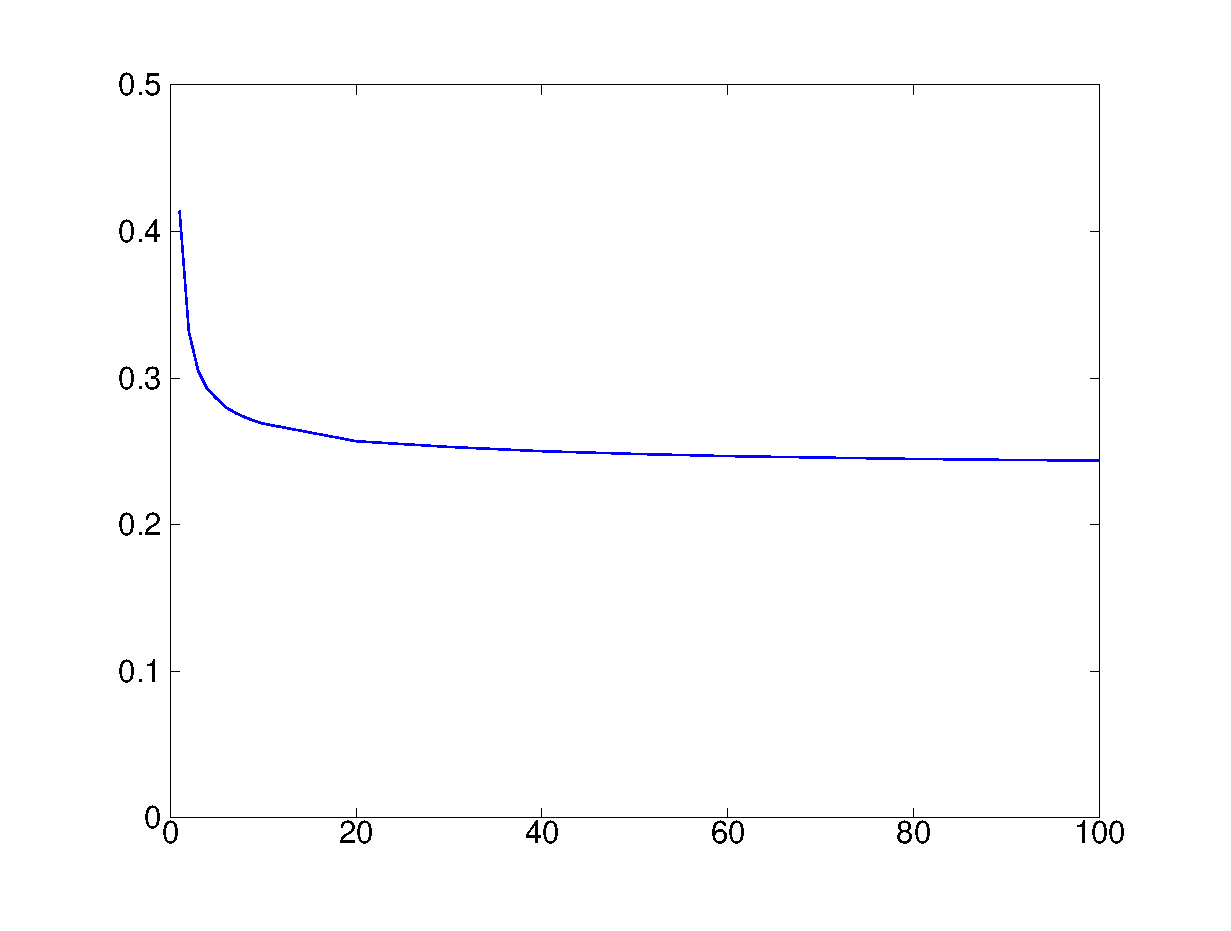
\includegraphics[width=0.9\textwidth]{figures/chi2_iters.eps}
\label{fig:chi2_iters}
\caption{The normalized $\chi^2$ error plotted against the number of minimization iterations.
    There is an exponential dropoff in improvement in $\chi^2$ as the number of iterations is
    increased. Based on this data set, we determined that gains of less than 0.005 were
    negligible (this is about where the slope begins to truly flatten out) and thus we stop
    iteration when the $\chi^2$ error does not decrease by more than 0.005.}
\end{figure}


\subsection*{B. $\chi^2$ Nearest Neighbor}

For this part, the robot was not given the ID for each landmark and therefore had to associate landmark observations on its own, using $\chi^2$ nearest neighbors.  In order to truly test the best associations for each of the new landmark observations, it would be necessary to create a set for every possible set of associations and find the set of associations that produced the lowest $\chi^2$.  A single association between one new observation and a previously seen landmark may have a positive increase in the $\chi^2$ value, but it may cause the other new observations to have such poor associations (or to become new landmarks), and therefore the overall system is worse than if a poorer first $\chi^2$ choice is made.  However, doing this many calculations would be very slow.  We therefore propose methods for mitigating this and share the changes we use in our code.

\subsubsection*{Optimization Proposals}
Nearest neighbors could be optimized by decreasing the number of computations required.  This could be done by decreasing the number of previously seen landmarks each new observations is compared to.  Additionally, the $\chi^2$ resulting from an association could be estimated by performing less Least-Squares iterations. We employed both of these methods in our code.

Another method to decrease computation would be to make assumptions about landmarks seen in sequential observations.  At each timestep one could consider the landmarks observed in each of the last several odometry positions.  For each of those landmarks, if the new observation approximately matches the position of that landmark, we can assume that it is the one being observed. In that case, the $\chi^2$ computation is skipped completely.

Another technique would be to use a variant of RANSAC to choose which observations are most likely to be the same landmark using $\chi^2$ estimate.

\subsubsection*{Our $\chi^2$ Nearest Neighbor Algorithm}
In our discussions about associating two landmarks, we determined that making false associations was a greater failure than not making a correct observation.  A few simple tests showed that a single incorrect association could result in a very large error.  As a result, our implementation seeks to be conservative about associating two landmarks.

We implemented $\chi^2$ nearest neighbor using both Euclidean distance and by considering the effect on the $\chi^2$ value of the system caused when associating each new landmark observation with each previous landmark observed.

Euclidean distance was used to minimize the number of possible landmark associations that would be considered.  Any landmark that was outside a threshold radius of the observed landmark location was ignored.  Since the $\chi^2$ nearest neighbor is more complex than calculating Euclidean distance, this is intended to decrease the computation time.  The threshold 5 was chosen to still allow a large area around the suspected location of the landmark to increase the likelihood of finding the correct association, should the robot's perceived self-location deviate greatly from its actual location.

Each previously observed landmark within the given area is considered for association using $\chi^2$ nearest neighbor.  Each association pair between a previous landmark and new observations is tested by assuming the association is correct and performing ten iterations of the Least-Squares Optimization loop. The resulting $\chi^2$ values are calculated.  We chose to do ten iterations because even very large initial $\chi^2$ begin to converge within ten iterations, although they may not reach their minimum, and iterating as much as in part A would lead to time-consuming steps.  The pair with the best resulting $\chi^2$ that falls within a given threshold change from the current $\chi^2$ is a associated.  The next best pair which does not include either of the already used landmarks is then associated (if it falls within the threshold).  This process is continued until all the new observations have either been associated with a previous landmark or there are no landmarks left within the threshold.  Any remaining new observations become new landmark poses.  The threshold we used was $max(1.2*old\chi^2, old\chi^2 + .5$).  This allowed $\chi^2$ increments proportional to the current $\chi^2$ value, which grows as more observations are made.

%\begin{algorithmic}   %%This was the old method.  Not sure that we want it anyway.
%\STATE{\bf Associate Landmarks}
%\STATE{\bf input:} list $newLandmarksObservations$
%\STATE{\bf output:} list $landmarksObserved$
%\FOR {every landmark in $newLandmarksObservations$}
%	\FOR{every  landmark in $previousLandmarksObservations$}
%		\IF{$distance(newLandmark, oldLandmark) < DIST\_THRESHOLD$}
%			\STATE Associate landmark and new landmark observation
%			\STATE Do 10 least-squares optimization iterations
%			\IF{$new\_chi^2 < max(CHI\_THRESHOLD*old\_chi^2, old\_ch1^2 + 1)$}
%				\STATE add $oldLandmark$ to $matchedList$
%			\ENDIF
%		\ENDIF
%	\ENDFOR
%	\IF{$matchedList$ is empty}
%		\STATE add $newLandmark$ to $landmarksObserved$
%	\ELSE
%		\STATE add $minChi^2(matchedList)$ to $landmarksObserved$
%	\ENDIF
%\ENDFOR
%\end{algorithmic}

\subsubsection*{Error Analysis}

\textcolor{red}{Put both errors in landmark associations and surface plot showing the number of data association errors as a function of odometry and measurement noise here.}

\begin{figure}[h!]
\centering
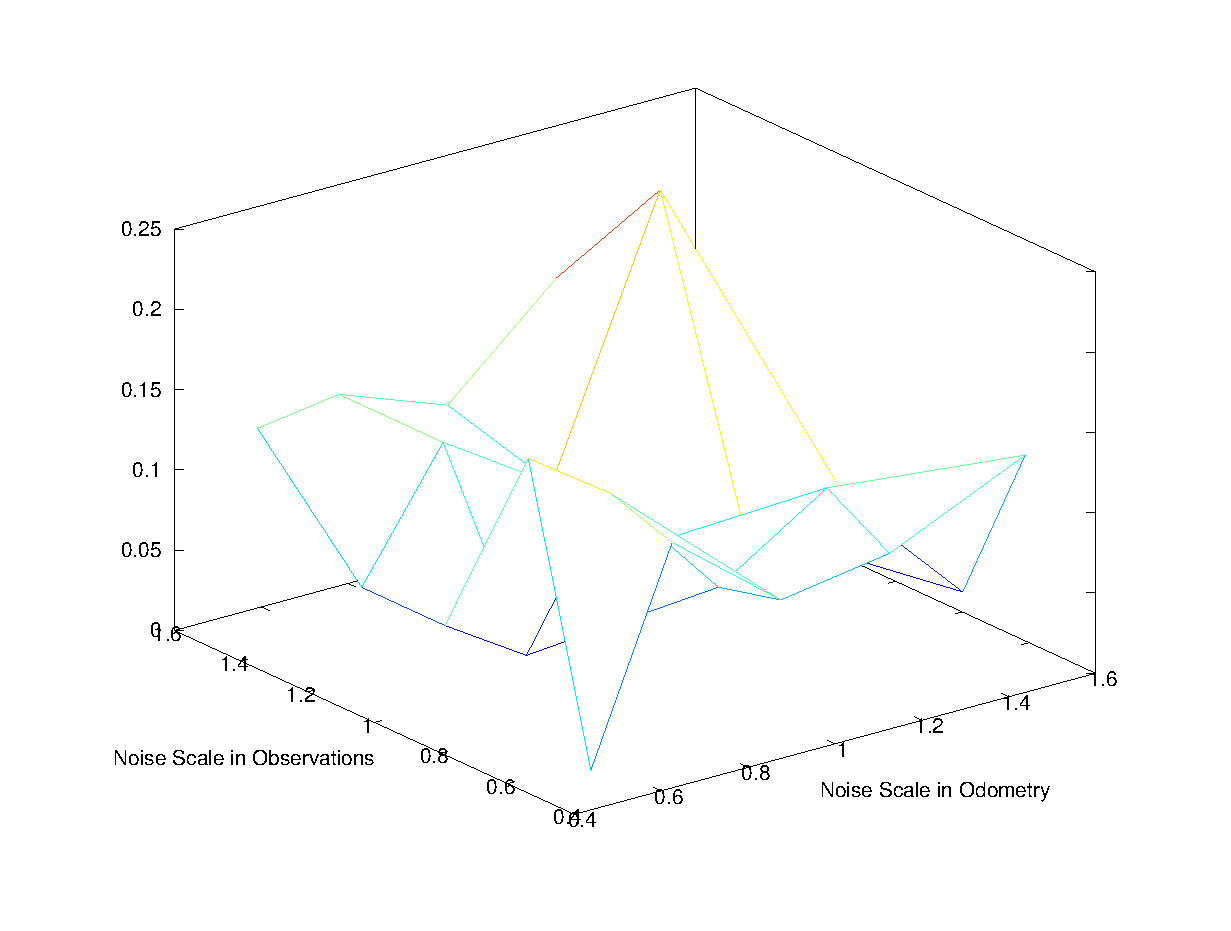
\includegraphics[width=0.9\textwidth]{figures/error_plot.eps}
\label{fig:assoc_err}
\caption{}%XXX}
\end{figure}

The four cases that can occur when trying to associate a landmark are:
\begin{itemize}
\item Incorrectly creating a new landmark (False Negative)
\item Incorrectly associating two landmarks (False Positive)
\item Correctly associating two landmarks (True Positive)
\item Correctly creating a new landmark (True Negative)
\end{itemize}

The surface plot showing the number of data association errors as a function of odometry and measurement noise is centered around the parameters given by Joho.  False negatives and false positives were combined for error.


\end{document}
